Das Buch {\em Lineare Algebra: Eine anwendungsorientierte Einführung}
wurde gemäss der Springer-Link Website in den ersten vier Monaten
nach Erscheinen (am 1.~September 2023) wie folgt heruntergeladen:
\begin{center}
\begin{tabular}{|>{$}l<{$}>{$}r<{$}|}
\hline
\text{Tage seit Erscheinen}&\text{Downloads (kumuliert)}\\
\hline
  30& 2866\\
  61& 5232\\
  91& 7266\\
 122& 8900\\
\hline
\end{tabular}
\end{center}
Formulieren Sie ein Modell für die Downloadzahlen und beantworten
Sie damit die folgenden Fragen.
\begin{teilaufgaben}
\item
Mit wievielen Downloads kann man innerhalb des ersten Jahres rechnen?
\item
An welchem Tag ist mit dem 10000sten Download zu rechnen?
\item
Wie gut ist Ihr Modell?
\end{teilaufgaben}

\begin{loesung}
\def\tabelle{
\begin{tabular}{|>{$}c<{$}|>{$}r<{$}|>{$}r<{$}|>{$}r<{$}|>{$}r<{$}|>{$}r<{$}|}
\hline
     i      &   x_i\phantom{.00}&       x_i^2\phantom{.00}&     y_i\phantom{.00}&        y_i^2\phantom{.00}&     x_iy_i\phantom{.00}\\
\hline
     1      &    30\phantom{.00}&         900\phantom{.00}&    2866\phantom{.00}&      8213956\phantom{.00}&      85980\phantom{.00}\\
     2      &    61\phantom{.00}&        3721\phantom{.00}&    5232\phantom{.00}&     27373824\phantom{.00}&     319152\phantom{.00}\\
     3      &    91\phantom{.00}&        8281\phantom{.00}&    7266\phantom{.00}&     52794756\phantom{.00}&     661206\phantom{.00}\\
     4      &   122\phantom{.00}&       14884\phantom{.00}&    8900\phantom{.00}&     79210000\phantom{.00}&    1085800\phantom{.00}\\
\hline
\text{Summe}&   304\phantom{.00}&       27786\phantom{.00}&   24264\phantom{.00}&    167592536\phantom{.00}&    2152138\phantom{.00}\\
\hline
E(\,\cdot\,)& 76.00&     6946.50& 6066.00&  41898134.00&  538034.50\\
\hline
\end{tabular}
}
\def\resultate{
\begin{align*}
\operatorname{var}(X)  &=    1170.50 & a &= \phantom{0}65.7997&&\\
\operatorname{var}(Y)  &= 5101778.00 & b &=           1065.2260&&\\
\operatorname{cov}(X,Y)&=   77018.50 & r &= \phantom{00}0.99666353&r^2&=0.99333820
\end{align*}
}
\def\aufgabea{
x = 365\qquad\Rightarrow\qquad y = a\cdot 365 + b = 25082.1012}
\def\awert{25.0821}
\def\aufgabeb{
10000 = ax+b\quad\Rightarrow\qquad x = \frac{10000-b}{a}= \frac{10000-1065.23}{65.80} = 135.79
}
\def\bwert{135.7875}
\def\aufgabec{
r^2=0.993338\quad\Rightarrow\quad r = 0.99666353
}
\def\punkte{
\punkt{30.0000}{2.8660}
\punkt{61.0000}{5.2320}
\punkt{91.0000}{7.2660}
\punkt{122.0000}{8.9000}
}
\def\gerade{
\draw[color=blue,line width=1pt] (0,{1.0652*\dy}) -- ({400*\dx},{27.3851*\dy});
}

\begin{figure}
\centering
\def\dx{0.03}
\def\dy{0.2}
\def\p#1#2{ ({(#1)*\dx},{(#2)*\dy}) }
\def\punkt#1#2{ \fill[color=red] \p{#1}{#2} circle[radius=0.1]; }
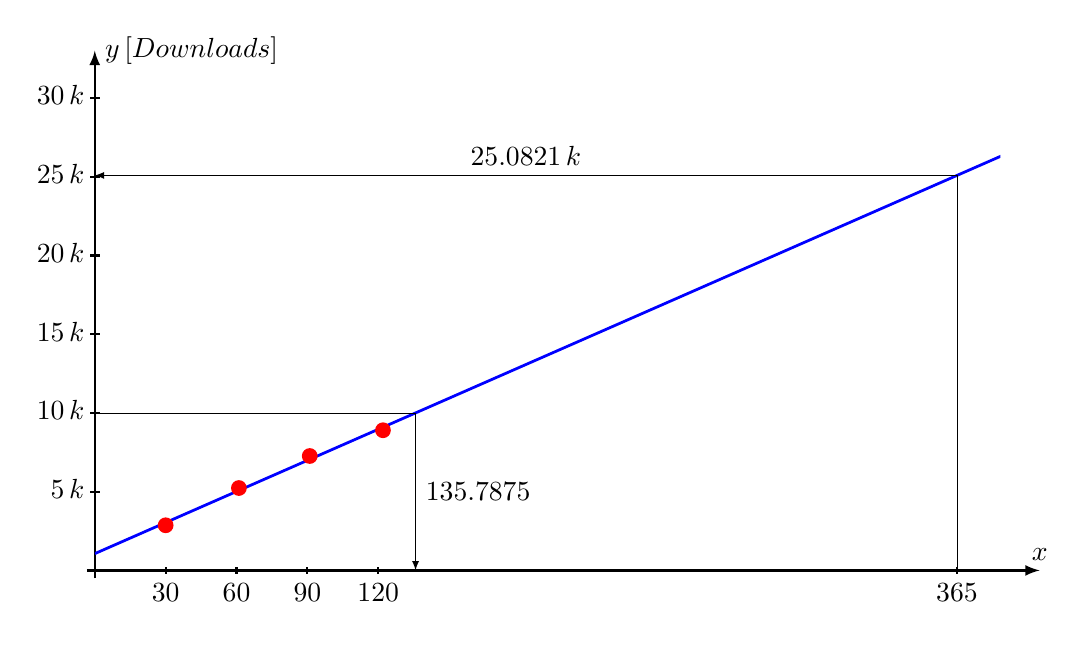
\begin{tikzpicture}[>=latex,thick]
\draw[->] (-0.1,0) -- (12,0) coordinate[label={$x$}];
\draw[->] (0,-0.1) -- (0,6.6) coordinate[label={right:$y\,\text{[Downloads]}$}];
\begin{scope}
	\clip (0,0) rectangle (11.5,6.0);
	\gerade
\end{scope}
\draw[->,line width=0.2pt] \p{365}{0} -- \p{365}{\awert} -- \p{0}{\awert};
\node at \p{(365/2)}{\awert} [above] {$\awert\,\text{k}$};
\draw[->,line width=0.2pt] \p{0}{10} -- \p{\bwert}{10} -- \p{\bwert}{0};
\node at \p{\bwert}{5} [right] {$\bwert$};
\foreach \x in {30,60,90,120,365}{
	\draw \p{\x}{-0.2} -- \p{\x}{0.2};
	\node at \p{\x}{0} [below] {$\x\mathstrut$};
}
\foreach \y in {5,10,...,30}{
	\draw \p{-2}{\y} -- \p{2}{\y};
	\node at \p{0}{\y} [left] {$\y\,\text{k}\mathstrut$};
}
\punkte
\end{tikzpicture}
\caption{Lineares Modell für Downloadzahlen in Abhängigkeit von der Zeit
seit Veröffentlichung am 1.~September 2023.
\label{40000053:fig}}
\end{figure}
Zur Berechnung der Koeffizienten $a$ und $b$ eines linearen Modells
$y=ax+b$
müssen die Zeitwerte $x_i$ und der Downloadzahlen $y_i$
und die Quadrate und gemischten Produkte gemittelt werden.
\begin{center}
\renewcommand\arraystretch{1.1}
\tabelle
\end{center}
Daraus können jetzt mit den bekannten Formeln die Varianzen, die
Kovarianz und die Koeffizienten bestimmt werden:
\resultate
\begin{teilaufgaben}
\item Zur Bestimmung der Downloads innerhalb eines Jahres berechnet man
die Vorhersage für $x=365$ und erhält
\[
\aufgabea.
\]
Man rechnet also mit etwa 25000 Downloads.
\item Es muss der $x$-Wert gefunden werden, für den $y=10000$ wird.
Dies geschieht durch Auflösen der Gleichung
\[
\aufgabeb.
\]
Mit 10000 Downloads ist also etwa im Januar zu rechnen.
\item
Da der Wert 
\[
\aufgabec
\]
sehr nahe bei $1$ liegt, ist die Qualität des Modells sehr gut.
\end{teilaufgaben}
Die Regressionsgerade ist in Abbildung~\ref{40000053:fig} dargestellt.
\end{loesung}

\begin{bewertung}
Lineare Regression ({\bf LR}) 1 Punkt,
Wert für Steigung ({\bf A}) 1 Punkt,
Wert für Achsabschnitt ({\bf B}) 1 Punkt,
Downloads in einem Jahr ({\bf D}) 1 Punkt,
Zeitpunkt für 10000 Downloads ({\bf X}) 1 Punkt,
Regressionskriterium ({\bf R}) 1 Punkt.
\end{bewertung}



